\chapter*{Le vélo\markboth{Le vélo}{}}
\section*{29 octobre 2014}
Mon objectif est de faire une bonne partie des déplacements en vélo, il me faut donc un vélo adapté au voyage :
\begin{itemize}
\item solide et fiable,
 \item réparable, donc avec des pièces standards,
 \item adapté à la route et aux chemins,
\item à un prix raisonnable.
\end{itemize}

 Les contacts que j'ai eu avec les vendeurs de vélos ne m'ont pas convaincu d'acheter un vélo tout prêt, ni d'en faire monter un sur mesure : prix élevés, configuration du vélo trop haut de gamme ou peu adapté. 
 
 J'ai choisi de monter le vélo en achetant toutes les pièces séparément, ce qui a l'avantage de me donner une bonne connaissance du vélo et du montage. Cela sera sans doute utile à un moment ou à un autre. 
 
 \newpage
 J'ai d'abord acheté un VTT d'occasion datant de 1992, principalement à cause du cadre en acier Tange, solide et réparable. En plus, j'ai gardé certaines autres pièces.

\begin{center}
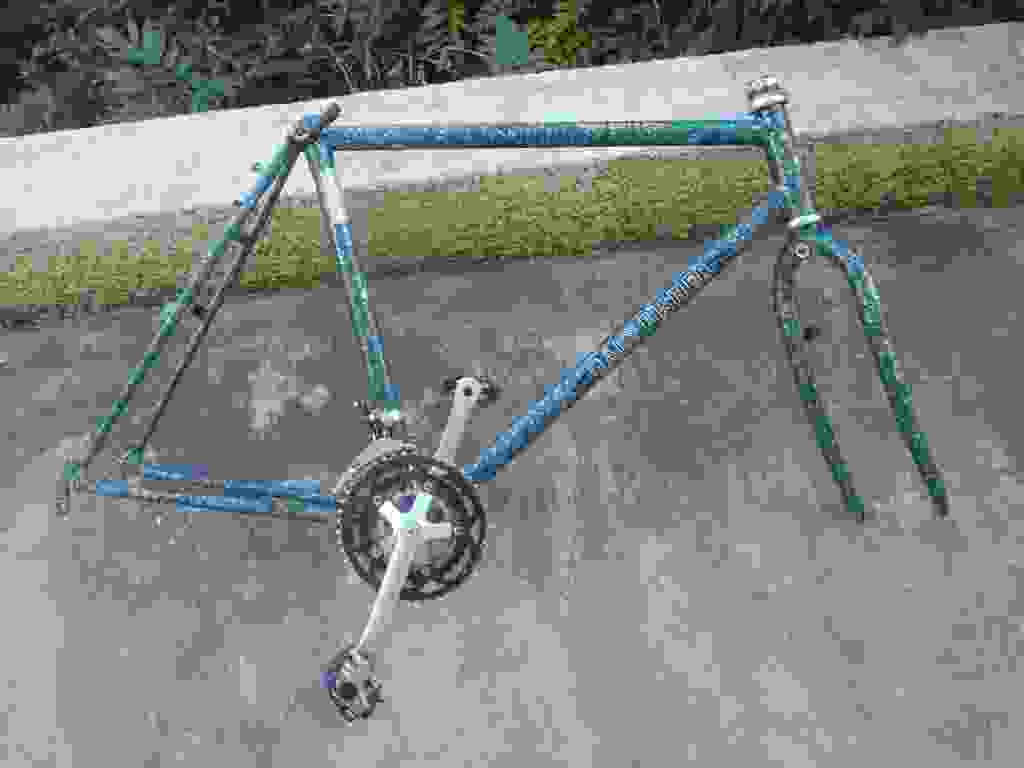
\includegraphics[width=\mywidth]{../wp-content/uploads/2014/10/Cadre.jpg} 
 \end{center}

 J'ai ensuite monté des pièces neuves, que j'ai choisies en m'appuyant sur les conseils que j'ai trouvés sur les blogs ou les forums. 
 
 Et le résultat : 
 
\begin{center}
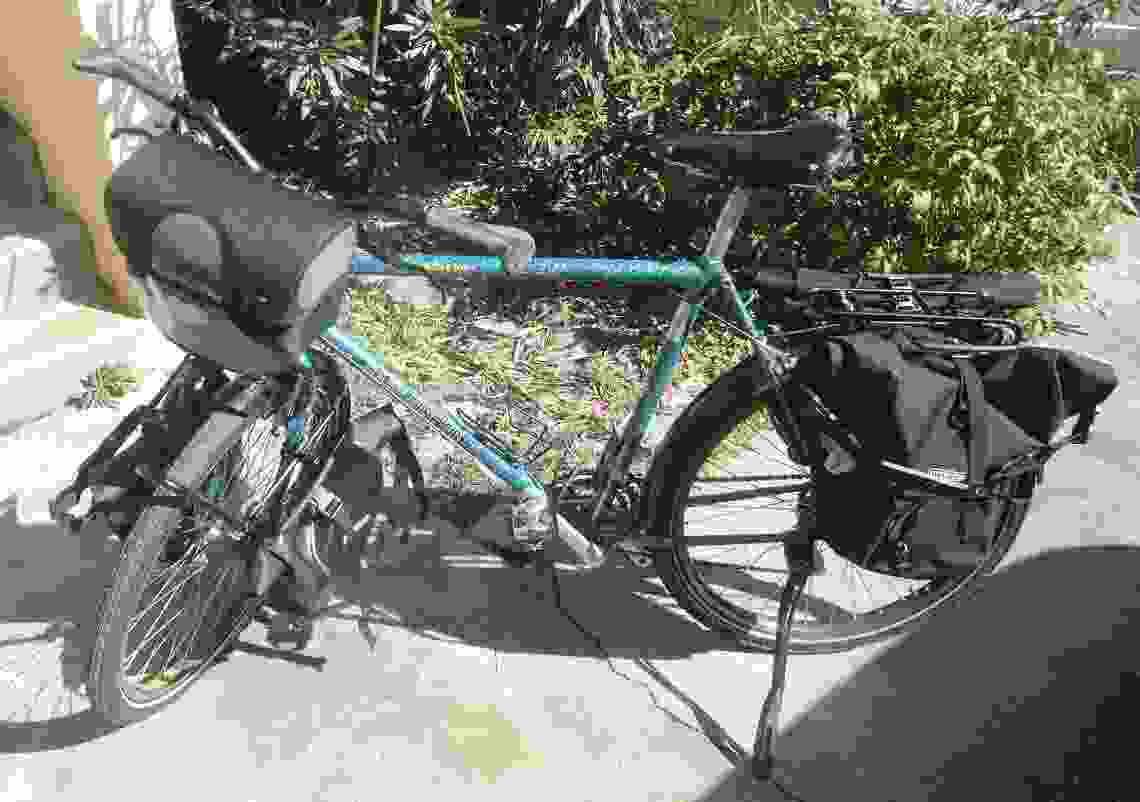
\includegraphics[width=\mywidth]{../wp-content/uploads/2014/10/Velo.jpg} 
\end{center}

 Ça donne un vélo complet pour environ 1000€, sacoches comprises. Voici le détail de la composition du vélo :
 \begin{center}
% \rowcolors{2}{white}{blue}
  \begin{tabular}{ll}
   \bf  Elément & \bf Modèle    \\ 
   \hline
  Cadre + fourche &  Gary Fisher (acier tange)    \\ 
  Jeu de direction &  D'origine du VTT    \\ 
  Potence + plongeur &  BBB Highrise 110mm    \\ 
  Cintre &  relevé XLC 63cm    \\  
  Poignées &  Ergonomique avec Bar End intégrés    \\   
  Transmission AV &  Shimano Deore LX d'origine du VTT    \\   
  Plateaux &  D'origine du VTT (petit plateau 24 dents)    \\   
  Transmission AR &  Shimano Acera 7 vitesses    \\   
  Roue libre AR &  7 vitesses 14-34 Megarange    \\   
  Chaine &  Shimano 6-8 vitesses    \\   
  Freins &  Shimano Acera V-Brake    \\   
  Pédalier &  D'origine du VTT    \\   
  Tige de selle &  D'origine du VTT    \\   
  Selle &  Brook B17 Imperial    \\   
  Roues &  Mavic d'origine du VTT (36 trous, montées main)    \\   
  Pneus &  Schwalbe Marathon Dureme  Mondial    \\   
  Bequille &  Pletscher ESGE    \\   
  Garde boue &  SKS Chromoplastics    \\   
  Porte bagages &  Tubus Tara  Logo    \\   
  Sacoches &  Ortlieb Back Roller, Front Roller, Ultimate 6 \\
  \hline
   \end{tabular}
   \end{center}
